\
% figures.tex — auto-generated by scripts/make_figures.py
% Insert \
% figures.tex — auto-generated by scripts/make_figures.py
% Insert \
% figures.tex — auto-generated by scripts/make_figures.py
% Insert \
% figures.tex — auto-generated by scripts/make_figures.py
% Insert \input{sections/figures} where desired in main.tex.
% DO NOT EDIT BY HAND — regenerate with: cert_env/bin/python scripts/make_figures.py

% -----------------------------------------------------------------------
\begin{figure}[tbp]
  \centering
  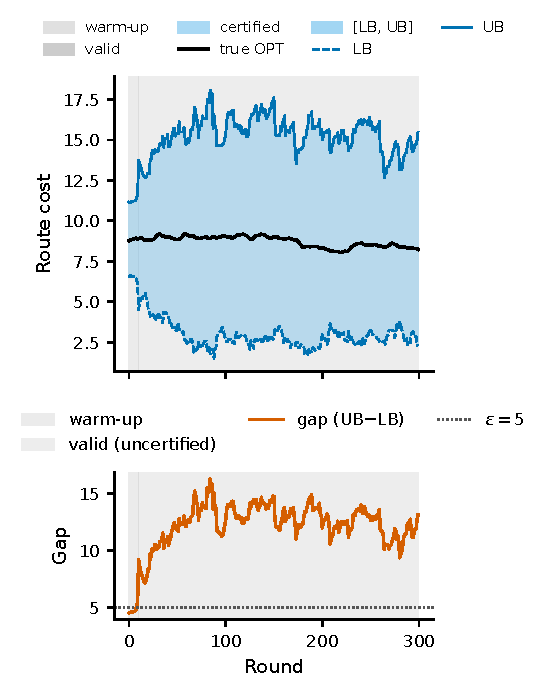
\includegraphics{figures/fig_gap_trajectory}
  \caption{Certificate gap trajectory for one representative episode
    (6$\times$6 grid, bounded drift $\rho{=}0.02$, \texttt{seed=3},
    default \textsc{cert} planner).
    \emph{Top}: true optimal cost OPT (black) overlaid on the $[\mathrm{LB},\mathrm{UB}]$
    certificate band (blue fill).  \emph{Bottom}: certificate gap $\mathrm{UB}{-}\mathrm{LB}$
    (red) and the target $\varepsilon{=}5$ (dotted).
    Shading: grey = warm-up (annealing claim below target),
    mid-grey = valid-uncertified, blue = certified ($\mathrm{gap}{\le}\varepsilon$).
    Single episode shown; aggregate over 25 seeds $\times$ 300 rounds is reported in
    Table~\ref{tab:tier0}.}
  \label{fig:gap_trajectory}
\end{figure}

% -----------------------------------------------------------------------
\begin{figure}[tbp]
  \centering
  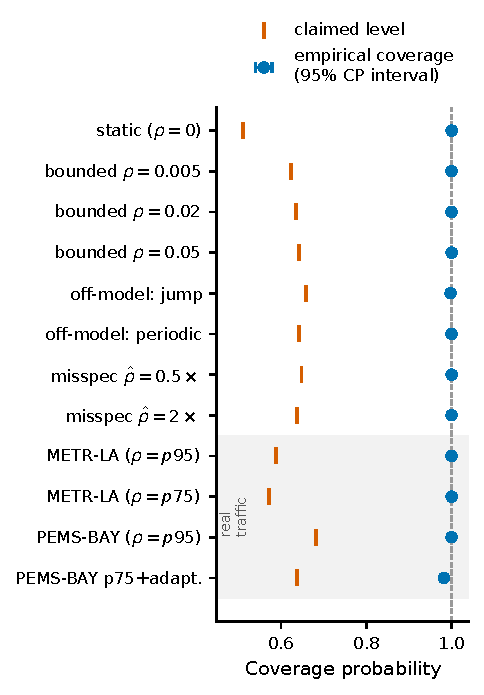
\includegraphics{figures/fig_coverage_vs_claim}
  \caption{Empirical coverage (filled circles, 95\% Clopper--Pearson bars) vs
    claimed confidence level (red tick marks) for eight synthetic conditions
    (white background) and four real-traffic conditions
    (grey background; METR-LA 20 days, PEMS-BAY 20 days).
    Synthetic: 25 seeds $\times$ 300 rounds, $6{\times}6$ grid, $\alpha'{=}0.2$.
    Coverage equals or exceeds the claim in every row; no row falls below
    the claimed level.}
  \label{fig:coverage_vs_claim}
\end{figure}

% -----------------------------------------------------------------------
\begin{figure}[tbp]
  \centering
  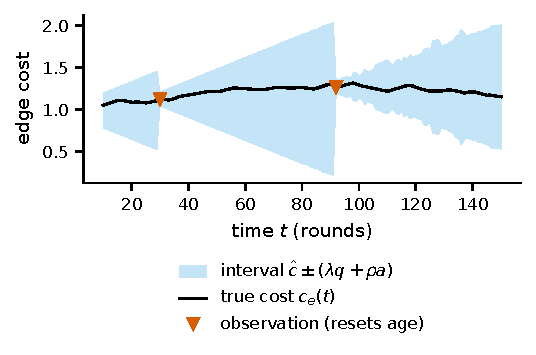
\includegraphics{figures/fig_interval_mechanism}
  \caption{The certificate's building block on one edge (bounded drift
    $\rho{=}0.02$, seed 7): the interval $\hat c \pm (\lambda q + \rho a)$
    (blue band) widens linearly with age $a$ and snaps tight when the edge
    is re-observed (red markers); the true cost (black) wanders within.
    Staleness is priced, not ignored.}
  \label{fig:interval_mechanism}
\end{figure}

% -----------------------------------------------------------------------
\begin{figure*}[tbp]
  \centering
  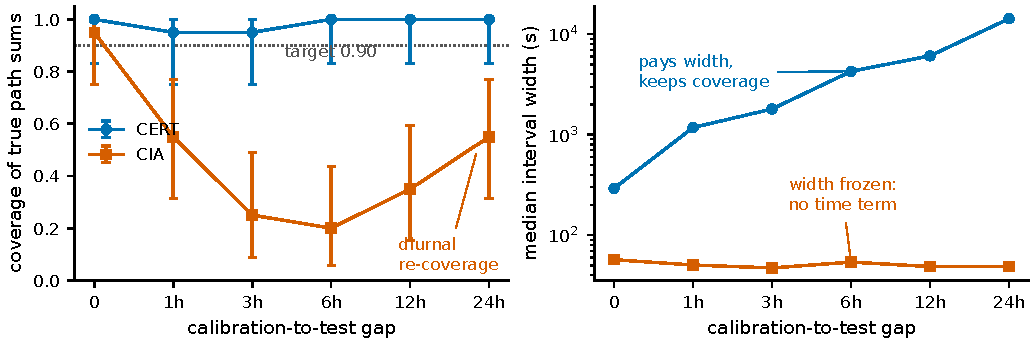
\includegraphics[width=\textwidth]{figures/fig_cia_collapse}
  \caption{Exchangeable conformal path sums (CIA~\citep{luo2024conformalized},
    their construction extracted and run on METR-LA; 50 paths $\times$ 20
    repetitions per gap, target 0.90) vs CERT as the calibration-to-test gap
    grows. \emph{Left}: CIA covers at gap 0 (its home setting) and collapses
    to 0.20--0.25 at the 3--6\,h staleness common in operation; the partial
    24\,h recovery is the diurnal cycle returning the network near its
    calibration state --- the failure mode is drift, not noise. CERT holds
    0.95--1.00 at every gap. \emph{Right}: the price, paid explicitly ---
    CIA's width is frozen ($\sim$50\,s, no time-dependent term) while CERT's
    $\rho\cdot$gap widening grows. Error bars: 95\% Clopper--Pearson.}
  \label{fig:cia_collapse}
\end{figure*}

% -----------------------------------------------------------------------
\begin{figure}[tbp]
  \centering
  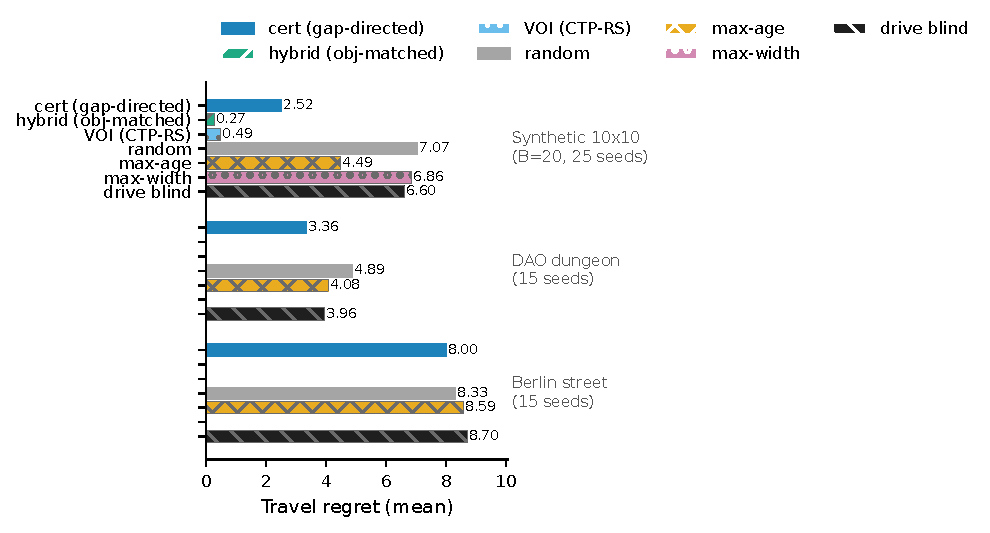
\includegraphics[width=0.92\textwidth]{figures/fig_regret_bars}
  \caption{Travel regret (mean, lower is better) by sensing policy across three
    map groups.
    \emph{Synthetic}: 10$\times$10 bounded drift $\rho{=}0.02$, budget $B{=}20$,
    25 seeds; includes hybrid (objective-matched, cert+VOI) and VOI (CTP-RS
    expected-route) policies from the external-baseline run (15 seeds).
    \emph{DAO dungeon / Berlin street}: MovingAI maps, 15 seeds,
    bounded drift $\rho{=}0.02$, $B{=}20$.
    Blank bars indicate conditions not run for that dataset.
    Regret is against a clairvoyant oracle replanning on true costs every step.}
  \label{fig:regret_bars}
\end{figure}

% -----------------------------------------------------------------------
\begin{figure}[tbp]
  \centering
  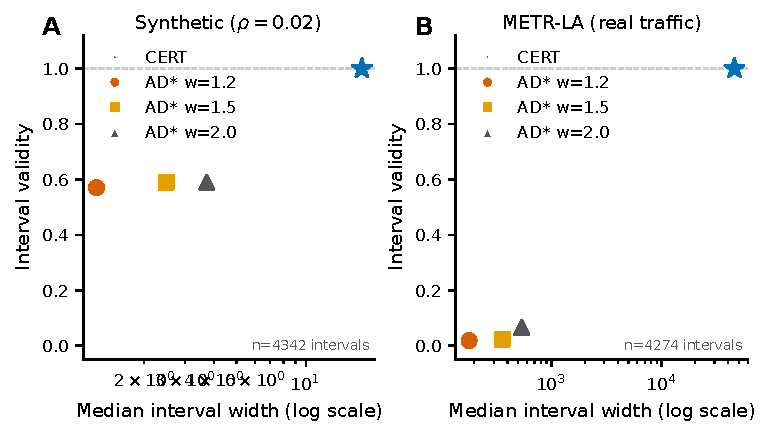
\includegraphics[width=0.8\textwidth]{figures/fig_bound_validity}
  \caption{Interval validity (fraction of rounds the true OPT lies inside the
    reported interval; $y$-axis) vs median interval width ($x$-axis, log scale)
    for \textsc{cert} and three AD$^*$-style inflation widths ($w\in\{1.2,1.5,2.0\}$),
    evaluated on a shared stale observation stream (neutral max-age sensing).
    \textbf{A}: synthetic bounded drift $\rho{=}0.02$ (15 seeds; $n=4340$ intervals per bound).
    \textbf{B}: METR-LA replayed traffic (15 seeds; $n=4273$).
    Narrow-and-wrong vs wide-and-sound is the observed trade-off:
    AD$^*$ semantics hedge search suboptimality, not map staleness.}
  \label{fig:bound_validity}
\end{figure}
 where desired in main.tex.
% DO NOT EDIT BY HAND — regenerate with: cert_env/bin/python scripts/make_figures.py

% -----------------------------------------------------------------------
\begin{figure}[tbp]
  \centering
  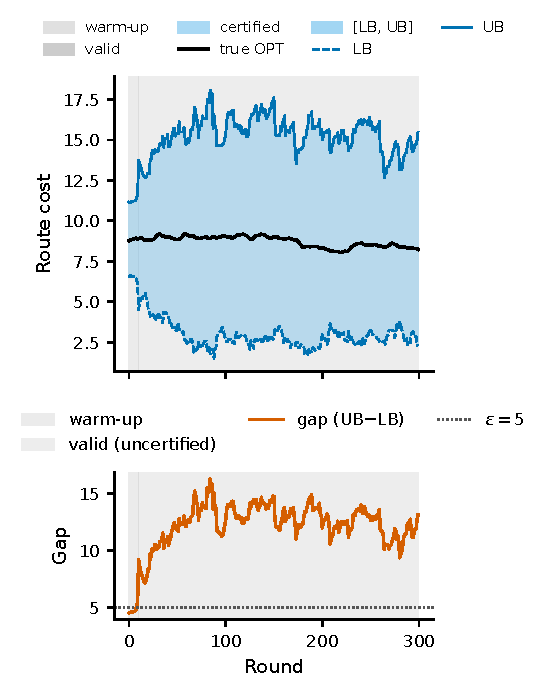
\includegraphics{figures/fig_gap_trajectory}
  \caption{Certificate gap trajectory for one representative episode
    (6$\times$6 grid, bounded drift $\rho{=}0.02$, \texttt{seed=3},
    default \textsc{cert} planner).
    \emph{Top}: true optimal cost OPT (black) overlaid on the $[\mathrm{LB},\mathrm{UB}]$
    certificate band (blue fill).  \emph{Bottom}: certificate gap $\mathrm{UB}{-}\mathrm{LB}$
    (red) and the target $\varepsilon{=}5$ (dotted).
    Shading: grey = warm-up (annealing claim below target),
    mid-grey = valid-uncertified, blue = certified ($\mathrm{gap}{\le}\varepsilon$).
    Single episode shown; aggregate over 25 seeds $\times$ 300 rounds is reported in
    Table~\ref{tab:tier0}.}
  \label{fig:gap_trajectory}
\end{figure}

% -----------------------------------------------------------------------
\begin{figure}[tbp]
  \centering
  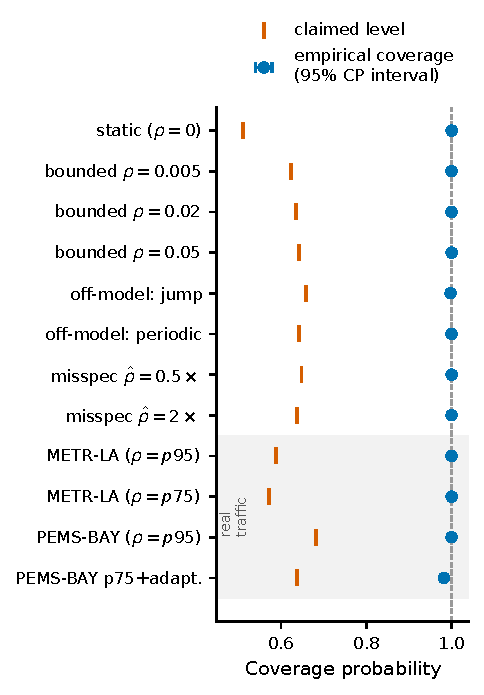
\includegraphics{figures/fig_coverage_vs_claim}
  \caption{Empirical coverage (filled circles, 95\% Clopper--Pearson bars) vs
    claimed confidence level (red tick marks) for eight synthetic conditions
    (white background) and four real-traffic conditions
    (grey background; METR-LA 20 days, PEMS-BAY 20 days).
    Synthetic: 25 seeds $\times$ 300 rounds, $6{\times}6$ grid, $\alpha'{=}0.2$.
    Coverage equals or exceeds the claim in every row; no row falls below
    the claimed level.}
  \label{fig:coverage_vs_claim}
\end{figure}

% -----------------------------------------------------------------------
\begin{figure}[tbp]
  \centering
  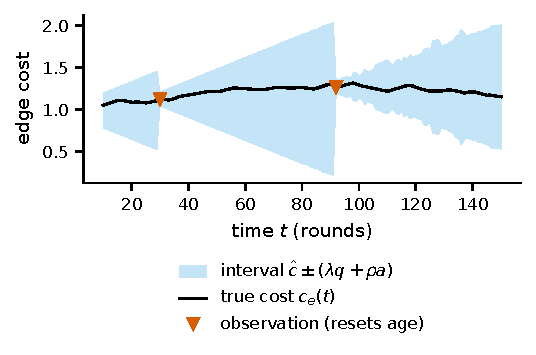
\includegraphics{figures/fig_interval_mechanism}
  \caption{The certificate's building block on one edge (bounded drift
    $\rho{=}0.02$, seed 7): the interval $\hat c \pm (\lambda q + \rho a)$
    (blue band) widens linearly with age $a$ and snaps tight when the edge
    is re-observed (red markers); the true cost (black) wanders within.
    Staleness is priced, not ignored.}
  \label{fig:interval_mechanism}
\end{figure}

% -----------------------------------------------------------------------
\begin{figure*}[tbp]
  \centering
  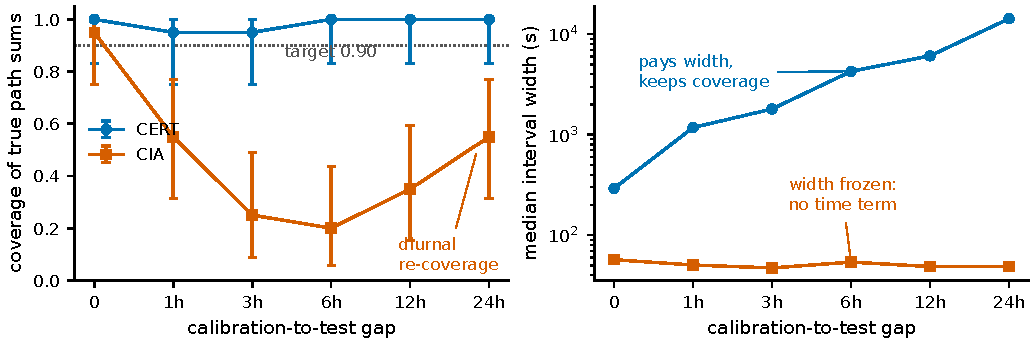
\includegraphics[width=\textwidth]{figures/fig_cia_collapse}
  \caption{Exchangeable conformal path sums (CIA~\citep{luo2024conformalized},
    their construction extracted and run on METR-LA; 50 paths $\times$ 20
    repetitions per gap, target 0.90) vs CERT as the calibration-to-test gap
    grows. \emph{Left}: CIA covers at gap 0 (its home setting) and collapses
    to 0.20--0.25 at the 3--6\,h staleness common in operation; the partial
    24\,h recovery is the diurnal cycle returning the network near its
    calibration state --- the failure mode is drift, not noise. CERT holds
    0.95--1.00 at every gap. \emph{Right}: the price, paid explicitly ---
    CIA's width is frozen ($\sim$50\,s, no time-dependent term) while CERT's
    $\rho\cdot$gap widening grows. Error bars: 95\% Clopper--Pearson.}
  \label{fig:cia_collapse}
\end{figure*}

% -----------------------------------------------------------------------
\begin{figure}[tbp]
  \centering
  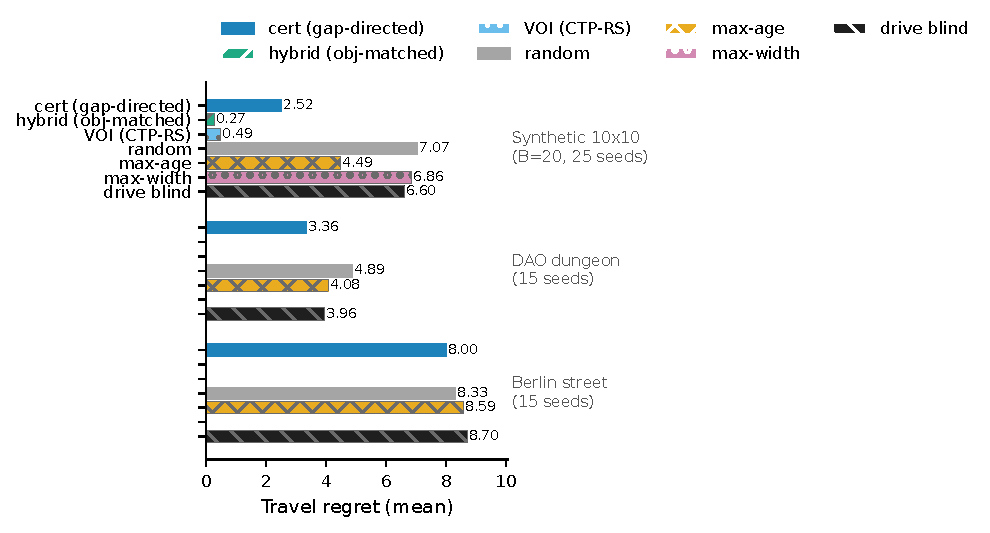
\includegraphics[width=0.92\textwidth]{figures/fig_regret_bars}
  \caption{Travel regret (mean, lower is better) by sensing policy across three
    map groups.
    \emph{Synthetic}: 10$\times$10 bounded drift $\rho{=}0.02$, budget $B{=}20$,
    25 seeds; includes hybrid (objective-matched, cert+VOI) and VOI (CTP-RS
    expected-route) policies from the external-baseline run (15 seeds).
    \emph{DAO dungeon / Berlin street}: MovingAI maps, 15 seeds,
    bounded drift $\rho{=}0.02$, $B{=}20$.
    Blank bars indicate conditions not run for that dataset.
    Regret is against a clairvoyant oracle replanning on true costs every step.}
  \label{fig:regret_bars}
\end{figure}

% -----------------------------------------------------------------------
\begin{figure}[tbp]
  \centering
  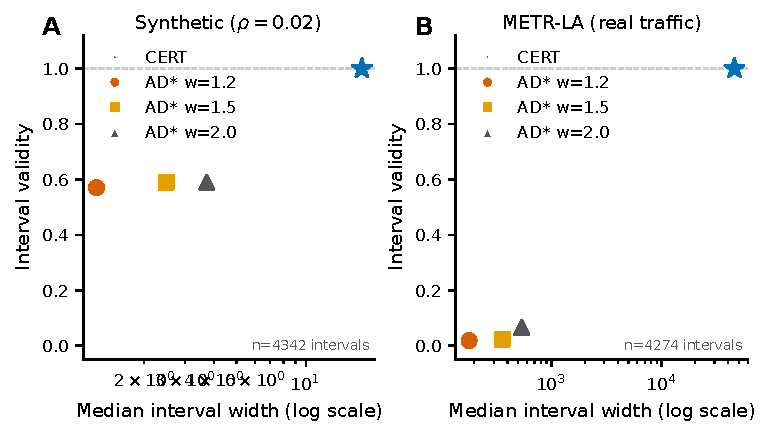
\includegraphics[width=0.8\textwidth]{figures/fig_bound_validity}
  \caption{Interval validity (fraction of rounds the true OPT lies inside the
    reported interval; $y$-axis) vs median interval width ($x$-axis, log scale)
    for \textsc{cert} and three AD$^*$-style inflation widths ($w\in\{1.2,1.5,2.0\}$),
    evaluated on a shared stale observation stream (neutral max-age sensing).
    \textbf{A}: synthetic bounded drift $\rho{=}0.02$ (15 seeds; $n=4340$ intervals per bound).
    \textbf{B}: METR-LA replayed traffic (15 seeds; $n=4273$).
    Narrow-and-wrong vs wide-and-sound is the observed trade-off:
    AD$^*$ semantics hedge search suboptimality, not map staleness.}
  \label{fig:bound_validity}
\end{figure}
 where desired in main.tex.
% DO NOT EDIT BY HAND — regenerate with: cert_env/bin/python scripts/make_figures.py

% -----------------------------------------------------------------------
\begin{figure}[tbp]
  \centering
  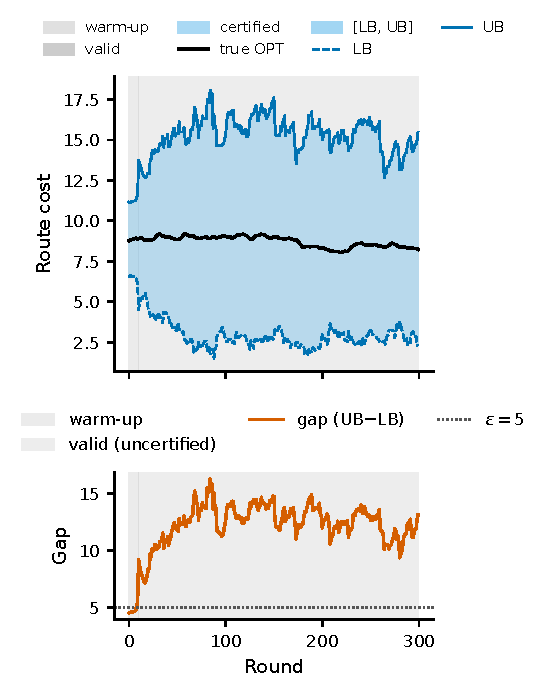
\includegraphics{figures/fig_gap_trajectory}
  \caption{Certificate gap trajectory for one representative episode
    (6$\times$6 grid, bounded drift $\rho{=}0.02$, \texttt{seed=3},
    default \textsc{cert} planner).
    \emph{Top}: true optimal cost OPT (black) overlaid on the $[\mathrm{LB},\mathrm{UB}]$
    certificate band (blue fill).  \emph{Bottom}: certificate gap $\mathrm{UB}{-}\mathrm{LB}$
    (red) and the target $\varepsilon{=}5$ (dotted).
    Shading: grey = warm-up (annealing claim below target),
    mid-grey = valid-uncertified, blue = certified ($\mathrm{gap}{\le}\varepsilon$).
    Single episode shown; aggregate over 25 seeds $\times$ 300 rounds is reported in
    Table~\ref{tab:tier0}.}
  \label{fig:gap_trajectory}
\end{figure}

% -----------------------------------------------------------------------
\begin{figure}[tbp]
  \centering
  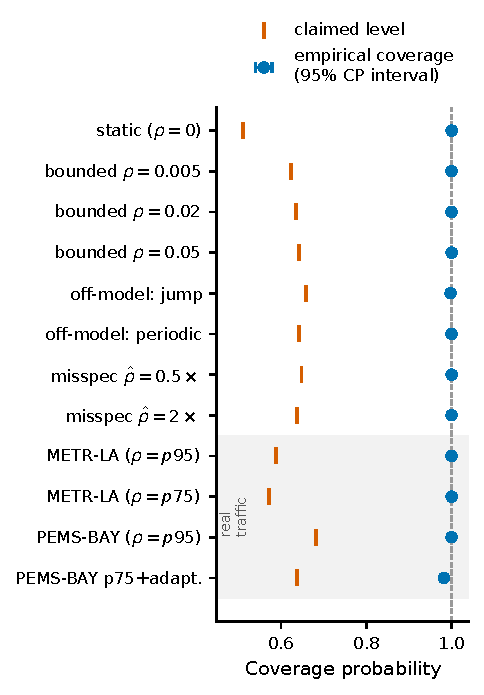
\includegraphics{figures/fig_coverage_vs_claim}
  \caption{Empirical coverage (filled circles, 95\% Clopper--Pearson bars) vs
    claimed confidence level (red tick marks) for eight synthetic conditions
    (white background) and four real-traffic conditions
    (grey background; METR-LA 20 days, PEMS-BAY 20 days).
    Synthetic: 25 seeds $\times$ 300 rounds, $6{\times}6$ grid, $\alpha'{=}0.2$.
    Coverage equals or exceeds the claim in every row; no row falls below
    the claimed level.}
  \label{fig:coverage_vs_claim}
\end{figure}

% -----------------------------------------------------------------------
\begin{figure}[tbp]
  \centering
  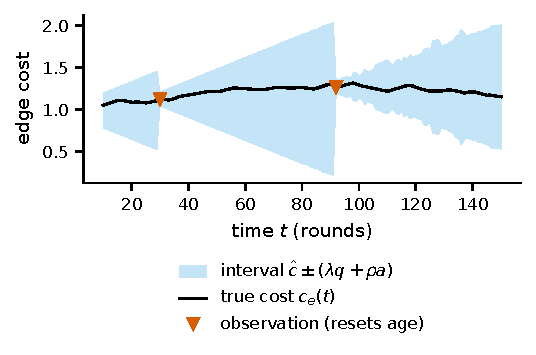
\includegraphics{figures/fig_interval_mechanism}
  \caption{The certificate's building block on one edge (bounded drift
    $\rho{=}0.02$, seed 7): the interval $\hat c \pm (\lambda q + \rho a)$
    (blue band) widens linearly with age $a$ and snaps tight when the edge
    is re-observed (red markers); the true cost (black) wanders within.
    Staleness is priced, not ignored.}
  \label{fig:interval_mechanism}
\end{figure}

% -----------------------------------------------------------------------
\begin{figure*}[tbp]
  \centering
  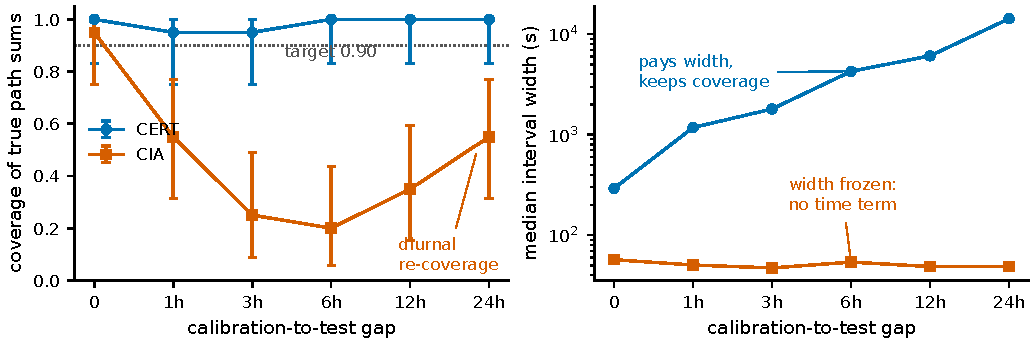
\includegraphics[width=\textwidth]{figures/fig_cia_collapse}
  \caption{Exchangeable conformal path sums (CIA~\citep{luo2024conformalized},
    their construction extracted and run on METR-LA; 50 paths $\times$ 20
    repetitions per gap, target 0.90) vs CERT as the calibration-to-test gap
    grows. \emph{Left}: CIA covers at gap 0 (its home setting) and collapses
    to 0.20--0.25 at the 3--6\,h staleness common in operation; the partial
    24\,h recovery is the diurnal cycle returning the network near its
    calibration state --- the failure mode is drift, not noise. CERT holds
    0.95--1.00 at every gap. \emph{Right}: the price, paid explicitly ---
    CIA's width is frozen ($\sim$50\,s, no time-dependent term) while CERT's
    $\rho\cdot$gap widening grows. Error bars: 95\% Clopper--Pearson.}
  \label{fig:cia_collapse}
\end{figure*}

% -----------------------------------------------------------------------
\begin{figure}[tbp]
  \centering
  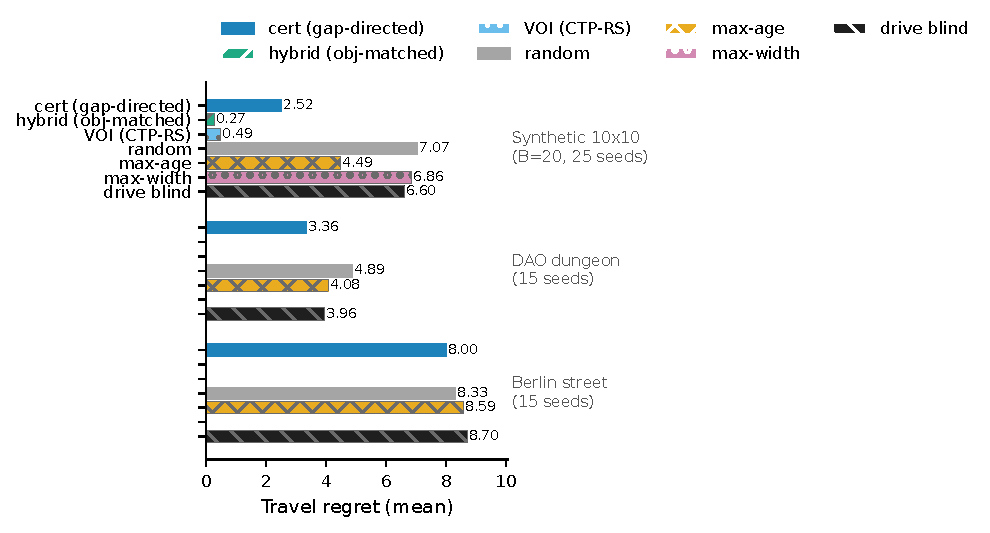
\includegraphics[width=0.92\textwidth]{figures/fig_regret_bars}
  \caption{Travel regret (mean, lower is better) by sensing policy across three
    map groups.
    \emph{Synthetic}: 10$\times$10 bounded drift $\rho{=}0.02$, budget $B{=}20$,
    25 seeds; includes hybrid (objective-matched, cert+VOI) and VOI (CTP-RS
    expected-route) policies from the external-baseline run (15 seeds).
    \emph{DAO dungeon / Berlin street}: MovingAI maps, 15 seeds,
    bounded drift $\rho{=}0.02$, $B{=}20$.
    Blank bars indicate conditions not run for that dataset.
    Regret is against a clairvoyant oracle replanning on true costs every step.}
  \label{fig:regret_bars}
\end{figure}

% -----------------------------------------------------------------------
\begin{figure}[tbp]
  \centering
  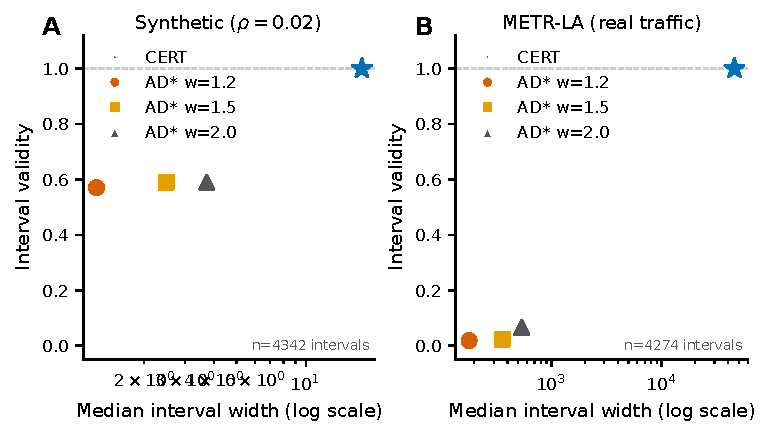
\includegraphics[width=0.8\textwidth]{figures/fig_bound_validity}
  \caption{Interval validity (fraction of rounds the true OPT lies inside the
    reported interval; $y$-axis) vs median interval width ($x$-axis, log scale)
    for \textsc{cert} and three AD$^*$-style inflation widths ($w\in\{1.2,1.5,2.0\}$),
    evaluated on a shared stale observation stream (neutral max-age sensing).
    \textbf{A}: synthetic bounded drift $\rho{=}0.02$ (15 seeds; $n=4340$ intervals per bound).
    \textbf{B}: METR-LA replayed traffic (15 seeds; $n=4273$).
    Narrow-and-wrong vs wide-and-sound is the observed trade-off:
    AD$^*$ semantics hedge search suboptimality, not map staleness.}
  \label{fig:bound_validity}
\end{figure}
 where desired in main.tex.
% DO NOT EDIT BY HAND — regenerate with: cert_env/bin/python scripts/make_figures.py

% -----------------------------------------------------------------------
\begin{figure}[tbp]
  \centering
  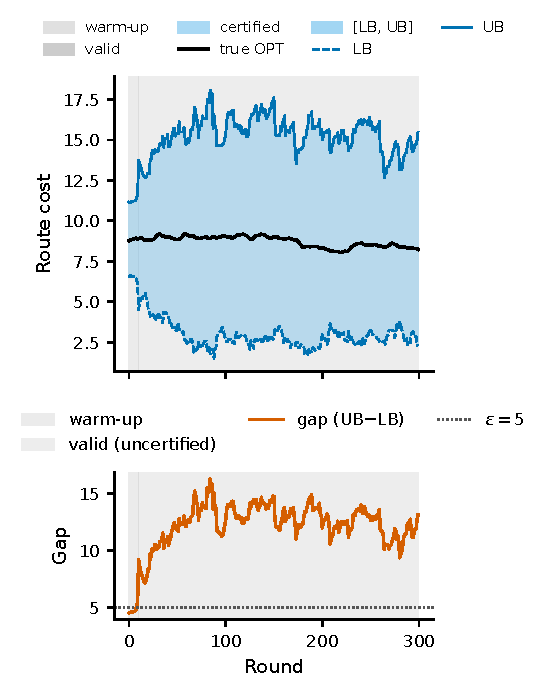
\includegraphics{figures/fig_gap_trajectory}
  \caption{Certificate gap trajectory for one representative episode
    (6$\times$6 grid, bounded drift $\rho{=}0.02$, \texttt{seed=3},
    default \textsc{cert} planner).
    \emph{Top}: true optimal cost OPT (black) overlaid on the $[\mathrm{LB},\mathrm{UB}]$
    certificate band (blue fill).  \emph{Bottom}: certificate gap $\mathrm{UB}{-}\mathrm{LB}$
    (red) and the target $\varepsilon{=}5$ (dotted).
    Shading: grey = warm-up (annealing claim below target),
    mid-grey = valid-uncertified, blue = certified ($\mathrm{gap}{\le}\varepsilon$).
    Single episode shown; aggregate over 25 seeds $\times$ 300 rounds is reported in
    Table~\ref{tab:tier0}.}
  \label{fig:gap_trajectory}
\end{figure}

% -----------------------------------------------------------------------
\begin{figure}[tbp]
  \centering
  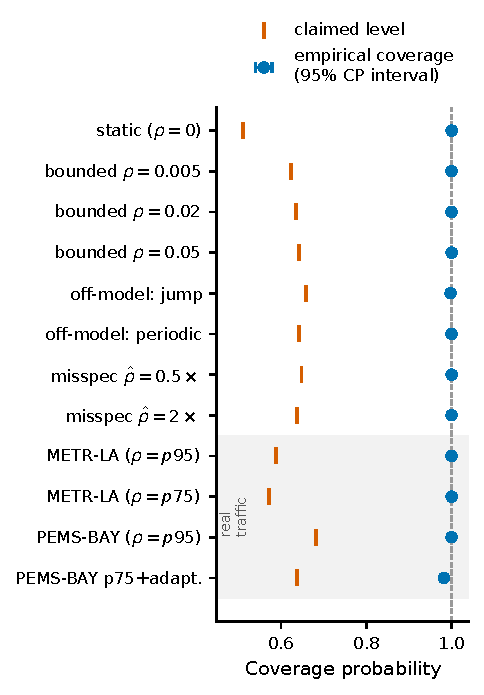
\includegraphics{figures/fig_coverage_vs_claim}
  \caption{Empirical coverage (filled circles, 95\% Clopper--Pearson bars) vs
    claimed confidence level (red tick marks) for eight synthetic conditions
    (white background) and four real-traffic conditions
    (grey background; METR-LA 20 days, PEMS-BAY 20 days).
    Synthetic: 25 seeds $\times$ 300 rounds, $6{\times}6$ grid, $\alpha'{=}0.2$.
    Coverage equals or exceeds the claim in every row; no row falls below
    the claimed level.}
  \label{fig:coverage_vs_claim}
\end{figure}

% -----------------------------------------------------------------------
\begin{figure}[tbp]
  \centering
  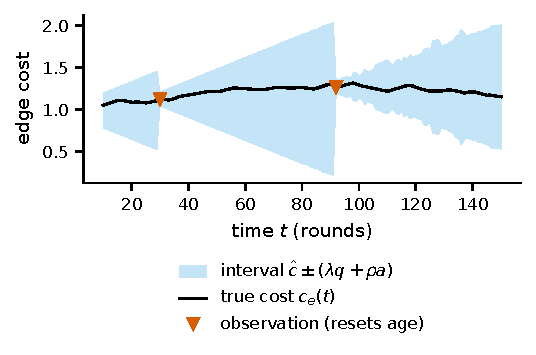
\includegraphics{figures/fig_interval_mechanism}
  \caption{The certificate's building block on one edge (bounded drift
    $\rho{=}0.02$, seed 7): the interval $\hat c \pm (\lambda q + \rho a)$
    (blue band) widens linearly with age $a$ and snaps tight when the edge
    is re-observed (red markers); the true cost (black) wanders within.
    Staleness is priced, not ignored.}
  \label{fig:interval_mechanism}
\end{figure}

% -----------------------------------------------------------------------
\begin{figure*}[tbp]
  \centering
  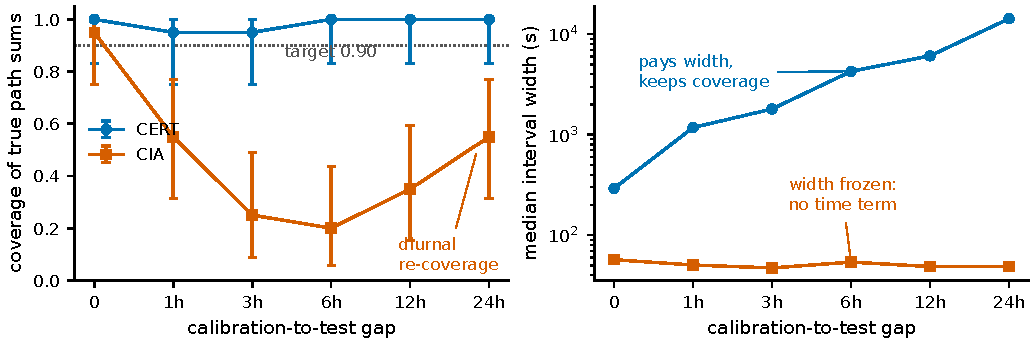
\includegraphics[width=\textwidth]{figures/fig_cia_collapse}
  \caption{Exchangeable conformal path sums (CIA~\citep{luo2024conformalized},
    their construction extracted and run on METR-LA; 50 paths $\times$ 20
    repetitions per gap, target 0.90) vs CERT as the calibration-to-test gap
    grows. \emph{Left}: CIA covers at gap 0 (its home setting) and collapses
    to 0.20--0.25 at the 3--6\,h staleness common in operation; the partial
    24\,h recovery is the diurnal cycle returning the network near its
    calibration state --- the failure mode is drift, not noise. CERT holds
    0.95--1.00 at every gap. \emph{Right}: the price, paid explicitly ---
    CIA's width is frozen ($\sim$50\,s, no time-dependent term) while CERT's
    $\rho\cdot$gap widening grows. Error bars: 95\% Clopper--Pearson.}
  \label{fig:cia_collapse}
\end{figure*}

% -----------------------------------------------------------------------
\begin{figure}[tbp]
  \centering
  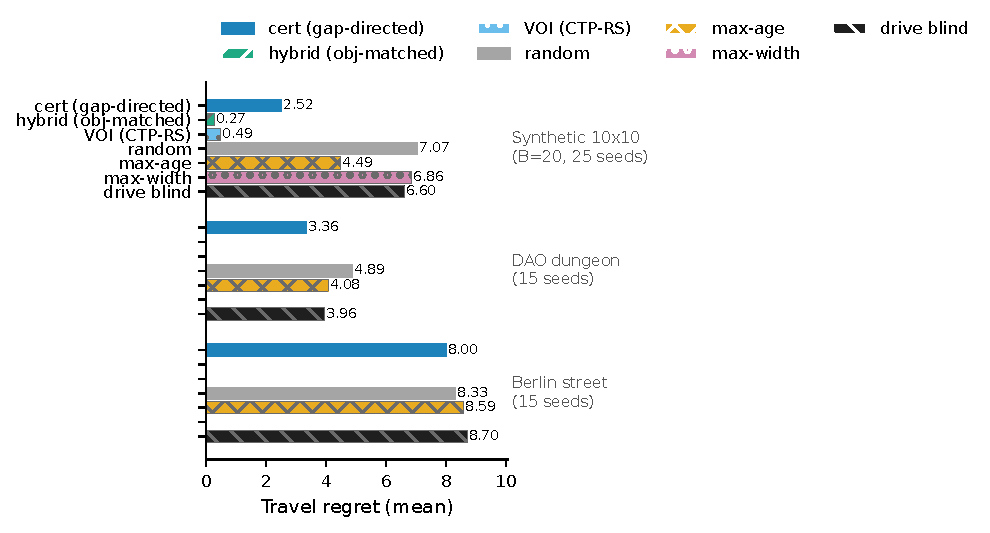
\includegraphics[width=0.92\textwidth]{figures/fig_regret_bars}
  \caption{Travel regret (mean, lower is better) by sensing policy across three
    map groups.
    \emph{Synthetic}: 10$\times$10 bounded drift $\rho{=}0.02$, budget $B{=}20$,
    25 seeds; includes hybrid (objective-matched, cert+VOI) and VOI (CTP-RS
    expected-route) policies from the external-baseline run (15 seeds).
    \emph{DAO dungeon / Berlin street}: MovingAI maps, 15 seeds,
    bounded drift $\rho{=}0.02$, $B{=}20$.
    Blank bars indicate conditions not run for that dataset.
    Regret is against a clairvoyant oracle replanning on true costs every step.}
  \label{fig:regret_bars}
\end{figure}

% -----------------------------------------------------------------------
\begin{figure}[tbp]
  \centering
  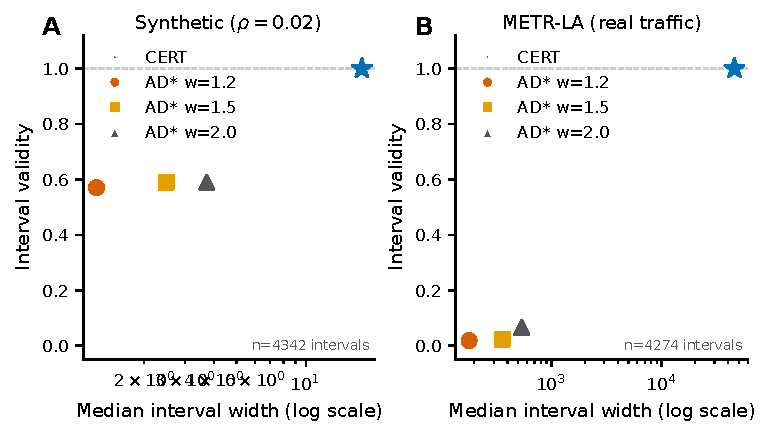
\includegraphics[width=0.8\textwidth]{figures/fig_bound_validity}
  \caption{Interval validity (fraction of rounds the true OPT lies inside the
    reported interval; $y$-axis) vs median interval width ($x$-axis, log scale)
    for \textsc{cert} and three AD$^*$-style inflation widths ($w\in\{1.2,1.5,2.0\}$),
    evaluated on a shared stale observation stream (neutral max-age sensing).
    \textbf{A}: synthetic bounded drift $\rho{=}0.02$ (15 seeds; $n=4340$ intervals per bound).
    \textbf{B}: METR-LA replayed traffic (15 seeds; $n=4273$).
    Narrow-and-wrong vs wide-and-sound is the observed trade-off:
    AD$^*$ semantics hedge search suboptimality, not map staleness.}
  \label{fig:bound_validity}
\end{figure}
